\section{Solving } 

\begin{frame}{}
    \tableofcontents[currentsection]
\end{frame}

\subsection{Solving Generalized Power Flow with Newton-Raphson}
\begin{frame}{Solving Generalized Power Flow with Newton-Raphson}
    To solve the generalized power flow problem, a set of known and unknown magnitudes must be defined. 
    \begin{itemize}
        \item Known magnitudes are those actively controlled by the system.
        \item Unknown magnitudes are not directly controlled.
    \end{itemize}
    The unknown set $x$ includes:
\[
x = [\delta, V, \textcolor{red}{\tau}, \textcolor{red}{m}, \textcolor{red}{P^\text{zip}}, \textcolor{red}{Q^\text{zip}}, \textcolor{red}{P_f}, \textcolor{red}{P_t}, \textcolor{red}{Q_f}, \textcolor{red}{Q_t}]^T
\]
\[
|x| = |\text{DC}|+ 2 \cdot |\text{AC}| + 3 \cdot |\text{VSC}| + 4 \cdot |\text{TR}|
\]


    This generalized formulation extends the traditional model by incorporating more unknowns, such as controlled transformers and AC/DC links.
\end{frame}

\subsection{Equations and Nodal Balance}
\begin{frame}{Equations and Nodal Balance (1)}
    The system of equations must balance the number of unknowns and equations. The nodal balance equations include:
    \begin{itemize}
        \item Nodal active and reactive power at AC buses.
        \item Active power at DC buses.
        \item Power loss equations for AC/DC links.
        \item Power equations for controlled transformers.
        \item Power equations for remotely-controlled passive branches.
    \end{itemize}
\end{frame}
\begin{frame}{Equations and Nodal Balance (2)}
    The system of equations is represented as:
    \begin{align*}
        g_{p,ac} &\coloneqq \sum P_i = 0 \quad \forall i \in \text{AC}, \\
        g_{q,ac} &\coloneqq \sum Q_i = 0 \quad \forall i \in \text{AC}, \\
        g_{p,dc} &\coloneqq \sum P_i = 0 \quad \forall i \in \text{DC}, \\
        g_{p,acdc} &\coloneqq P_{fk}^\text{acdc} + P_{tk}^\text{acdc} - P_{\text{loss},k}^\text{acdc} = 0 \quad \forall k \in ACDC. \\
        g_{p_f,tr} &\coloneqq P_{fk}^\text{tr} = f(\delta, V, \tau, m) \quad \forall k \in TR, \\
        g_{p_t,tr} &\coloneqq P_{tk}^\text{tr} = f(\delta, V, \tau, m) \quad \forall k \in TR, \\
        g_{q_f,tr} &\coloneqq Q_{fk}^\text{tr} = f(\delta, V, \tau, m) \quad \forall k \in TR, \\
        g_{q_t,tr} &\coloneqq Q_{tk}^\text{tr} = f(\delta, V, \tau, m) \quad \forall k \in TR, \\
        g_{p_{ij}, \kappa } \coloneqq P_{ij} &= \Re \{ V_i \cdot (V_i - V_j)^* \cdot Y^*_{ij} \} \quad \forall b \in \mathcal{B}_{p_{ij}, \kappa} \\
        g_{q_{ij}, \kappa } \coloneqq Q_{ij} &= \Im \{ V_i \cdot (V_i - V_j)^* \cdot Y^*_{ij} \} \quad \forall b \in \mathcal{B}_{q_{ij}, \kappa} \\
        g_{p_{ji}, \kappa } \coloneqq P_{ji} &= \Re \{ V_j \cdot (V_j - V_i)^* \cdot Y^*_{ij} \} \quad \forall b \in \mathcal{B}_{p_{ji}, \kappa} \\
        g_{q_{ji}, \kappa } \coloneqq Q_{ji} &= \Im \{ V_j \cdot (V_j - V_i)^* \cdot Y^*_{ij} \} \quad \forall b \in \mathcal{B}_{q_{ji}, \kappa}
    \end{align*}
\end{frame}

\begin{frame}{Tracking Known and Unknown Magnitudes}
    Sets are used to track known and unknown magnitudes for bus and branch variables:
    
    \begin{table}[!htb]
    \centering
    \caption{Sets for identifying known and unknown magnitudes.}
    \begin{tabular}{cl}
        \hline
        \textbf{Set} & \textbf{Description} \\
        \hline
        $I_{\delta}$ & Known bus voltage phase \\
        $I_{V}$ & Known bus voltage magnitudes \\
        $I_{p}$ & Known bus ZIP active powers \\
        $I_{q}$ & Known bus ZIP reactive powers \\
        $K_{\tau}$ & Known branch tap phase shift angles \\
        $K_{m}$ & Known branch tap ratios \\
        $\overline{I}_{\delta}$ & Unknown bus voltage phase \\
        $\overline{I}_{V}$ & Unknown bus voltage magnitudes \\
        \dots & \dots \\
        \hline
    \end{tabular}
    \label{tab:setsver2}
    \end{table}
\end{frame}

\begin{frame}{Indices and Subsystems}
    We devised an algorithm based on Depth-First Search (DFS) to systematically create sets of indices for the generalized power flow method. The key steps include:
    \begin{itemize}
        \item Initialise indices as unknowns when active elements are added to the grid.
        \item Move indices to known sets as active elements assert control.
        \item Separate AC and DC subsystems by removing AC/DC links.
        \item Identify connected components (subsystems) in the grid.
        \item Select references within each subsystem.
    \end{itemize}
\end{frame}


\begin{frame}{Constructing the Jacobian Matrix}
    To solve the system using the Newton-Raphson method, the Jacobian matrix is constructed. This matrix contains the partial derivatives of the system of equations with respect to the unknown variables.
    
    The typical Newton-Raphson system is represented as:
    \[
        \mathbf{J} \Delta \mathbf{x} = -\mathbf{g}
    \]
    where:
    \begin{itemize}
        \item $\mathbf{J}$ is the Jacobian matrix.
        \item $\Delta \mathbf{x}$ is the vector of unknowns.
        \item $\mathbf{g}$ is the residual vector of equations.
    \end{itemize}
\end{frame}
\begin{frame}{Jacobian Variables}
    The unknown vector $\Delta \mathbf{x}$ is represented as:
    \[
    \Delta \mathbf{x} =
    [\Delta \delta, \Delta V, \Delta \tau, \Delta m, \Delta P^\text{zip}, \Delta Q^\text{zip}, \Delta P_f, \Delta P_t, \Delta Q_f, \Delta Q_t]^T
    \]
    The residual vector $\mathbf{g}$ is:
    \[
    \mathbf{g} =
    [g_{p,ac}, g_{q,ac}, g_{p,dc}, g_{p,acdc}, g_{p_f,tr}, g_{p_t,tr}, g_{q_f,tr}, g_{q_t,tr}, g_{p_{ij}, \kappa}, g_{q_{ij}, \kappa}, g_{p_{ji}, \kappa}, g_{q_{ji}, \kappa}]^T
    \]
\end{frame}


\begin{frame}{Jacobian Matrix in Full}
    \scriptsize  % Shrinks the font size to make it fit better on the slide
    The full Jacobian matrix $\mathbf{J}$ is constructed as follows, showing the partial derivatives of the equations with respect to the unknown variables:
    
    \[
    \mathbf{J} = 
    \begin{bmatrix}
        \frac{\partial g_{p,ac}}{\partial \delta} & \frac{\partial g_{p,ac}}{\partial V} & \frac{\partial g_{p,ac}}{\partial \tau} & \frac{\partial g_{p,ac}}{\partial m} & \frac{\partial g_{p,ac}}{\partial P^\text{zip}} & \frac{\partial g_{p,ac}}{\partial Q^\text{zip}} & \frac{\partial g_{p,ac}}{\partial P_f} & \frac{\partial g_{p,ac}}{\partial P_t} & \frac{\partial g_{p,ac}}{\partial Q_f} & \frac{\partial g_{p,ac}}{\partial Q_t} \\
        \frac{\partial g_{q,ac}}{\partial \delta} & \frac{\partial g_{q,ac}}{\partial V} & \frac{\partial g_{q,ac}}{\partial \tau} & \frac{\partial g_{q,ac}}{\partial m} & \frac{\partial g_{q,ac}}{\partial P^\text{zip}} & \frac{\partial g_{q,ac}}{\partial Q^\text{zip}} & \frac{\partial g_{q,ac}}{\partial P_f} & \frac{\partial g_{q,ac}}{\partial P_t} & \frac{\partial g_{q,ac}}{\partial Q_f} & \frac{\partial g_{q,ac}}{\partial Q_t} \\
        \frac{\partial g_{p,dc}}{\partial \delta} & \frac{\partial g_{p,dc}}{\partial V} & \frac{\partial g_{p,dc}}{\partial \tau} & \frac{\partial g_{p,dc}}{\partial m} & \frac{\partial g_{p,dc}}{\partial P^\text{zip}} & \frac{\partial g_{p,dc}}{\partial Q^\text{zip}} & \frac{\partial g_{p,dc}}{\partial P_f} & \frac{\partial g_{p,dc}}{\partial P_t} & \frac{\partial g_{p,dc}}{\partial Q_f} & \frac{\partial g_{p,dc}}{\partial Q_t} \\
        \frac{\partial g_{p,acdc}}{\partial \delta} & \frac{\partial g_{p,acdc}}{\partial V} & \frac{\partial g_{p,acdc}}{\partial \tau} & \frac{\partial g_{p,acdc}}{\partial m} & \frac{\partial g_{p,acdc}}{\partial P^\text{zip}} & \frac{\partial g_{p,acdc}}{\partial Q^\text{zip}} & \frac{\partial g_{p,acdc}}{\partial P_f} & \frac{\partial g_{p,acdc}}{\partial P_t} & \frac{\partial g_{p,acdc}}{\partial Q_f} & \frac{\partial g_{p,acdc}}{\partial Q_t} \\
        \frac{\partial g_{p_f,tr}}{\partial \delta} & \frac{\partial g_{p_f,tr}}{\partial V} & \frac{\partial g_{p_f,tr}}{\partial \tau} & \frac{\partial g_{p_f,tr}}{\partial m} & \frac{\partial g_{p_f,tr}}{\partial P^\text{zip}} & \frac{\partial g_{p_f,tr}}{\partial Q^\text{zip}} & \frac{\partial g_{p_f,tr}}{\partial P_f} & \frac{\partial g_{p_f,tr}}{\partial P_t} & \frac{\partial g_{p_f,tr}}{\partial Q_f} & \frac{\partial g_{p_f,tr}}{\partial Q_t} \\
        \frac{\partial g_{p_t,tr}}{\partial \delta} & \frac{\partial g_{p_t,tr}}{\partial V} & \frac{\partial g_{p_t,tr}}{\partial \tau} & \frac{\partial g_{p_t,tr}}{\partial m} & \frac{\partial g_{p_t,tr}}{\partial P^\text{zip}} & \frac{\partial g_{p_t,tr}}{\partial Q^\text{zip}} & \frac{\partial g_{p_t,tr}}{\partial P_f} & \frac{\partial g_{p_t,tr}}{\partial P_t} & \frac{\partial g_{p_t,tr}}{\partial Q_f} & \frac{\partial g_{p_t,tr}}{\partial Q_t} \\
        \frac{\partial g_{q_f,tr}}{\partial \delta} & \frac{\partial g_{q_f,tr}}{\partial V} & \frac{\partial g_{q_f,tr}}{\partial \tau} & \frac{\partial g_{q_f,tr}}{\partial m} & \frac{\partial g_{q_f,tr}}{\partial P^\text{zip}} & \frac{\partial g_{q_f,tr}}{\partial Q^\text{zip}} & \frac{\partial g_{q_f,tr}}{\partial P_f} & \frac{\partial g_{q_f,tr}}{\partial P_t} & \frac{\partial g_{q_f,tr}}{\partial Q_f} & \frac{\partial g_{q_f,tr}}{\partial Q_t} \\
        \frac{\partial g_{q_t,tr}}{\partial \delta} & \frac{\partial g_{q_t,tr}}{\partial V} & \frac{\partial g_{q_t,tr}}{\partial \tau} & \frac{\partial g_{q_t,tr}}{\partial m} & \frac{\partial g_{q_t,tr}}{\partial P^\text{zip}} & \frac{\partial g_{q_t,tr}}{\partial Q^\text{zip}} & \frac{\partial g_{q_t,tr}}{\partial P_f} & \frac{\partial g_{q_t,tr}}{\partial P_t} & \frac{\partial g_{q_t,tr}}{\partial Q_f} & \frac{\partial g_{q_t,tr}}{\partial Q_t} \\
        \frac{\partial g_{pf, \kappa }}{\partial \delta} & \frac{\partial g_{pf, \kappa }}{\partial V} & \frac{\partial g_{pf, \kappa }}{\partial \tau} & \frac{\partial g_{pf, \kappa }}{\partial m} & \frac{\partial g_{pf, \kappa }}{\partial P^\text{zip}} & \frac{\partial g_{pf, \kappa }}{\partial Q^\text{zip}} & \frac{\partial g_{pf, \kappa }}{\partial P_f} & \frac{\partial g_{pf, \kappa }}{\partial P_t} & \frac{\partial g_{pf, \kappa }}{\partial Q_f} & \frac{\partial g_{pf, \kappa }}{\partial Q_t} \\
        \frac{\partial g_{qf, \kappa }}{\partial \delta} & \frac{\partial g_{qf, \kappa }}{\partial V} & \frac{\partial g_{qf, \kappa }}{\partial \tau} & \frac{\partial g_{qf, \kappa }}{\partial m} & \frac{\partial g_{qf, \kappa }}{\partial P^\text{zip}} & \frac{\partial g_{qf, \kappa }}{\partial Q^\text{zip}} & \frac{\partial g_{qf, \kappa }}{\partial P_f} & \frac{\partial g_{qf, \kappa }}{\partial P_t} & \frac{\partial g_{qf, \kappa }}{\partial Q_f} & \frac{\partial g_{qf, \kappa }}{\partial Q_t} \\
        \frac{\partial g_{pt, \kappa }}{\partial \delta} & \frac{\partial g_{pt, \kappa }}{\partial V} & \frac{\partial g_{pt, \kappa }}{\partial \tau} & \frac{\partial g_{pt, \kappa }}{\partial m} & \frac{\partial g_{pt, \kappa }}{\partial P^\text{zip}} & \frac{\partial g_{pt, \kappa }}{\partial Q^\text{zip}} & \frac{\partial g_{pt, \kappa }}{\partial P_f} & \frac{\partial g_{pt, \kappa }}{\partial P_t} & \frac{\partial g_{pt, \kappa }}{\partial Q_f} & \frac{\partial g_{pt, \kappa }}{\partial Q_t} \\
        \frac{\partial g_{qt, \kappa }}{\partial \delta} & \frac{\partial g_{qt, \kappa }}{\partial V} & \frac{\partial g_{qt, \kappa }}{\partial \tau} & \frac{\partial g_{qt, \kappa }}{\partial m} & \frac{\partial g_{qt, \kappa }}{\partial P^\text{zip}} & \frac{\partial g_{qt, \kappa }}{\partial Q^\text{zip}} & \frac{\partial g_{qt, \kappa }}{\partial P_f} & \frac{\partial g_{qt, \kappa }}{\partial P_t} & \frac{\partial g_{qt, \kappa }}{\partial Q_f} & \frac{\partial g_{qt, \kappa }}{\partial Q_t}
    \end{bmatrix}
    \]
\end{frame}




\begin{frame}{General Rules for Solvability}
    \begin{columns}
        % Left column with the rules
        \begin{column}{0.5\textwidth}
            To ensure solvability in generalized power flow, the following rules are defined:
            \begin{itemize}
                \item Each subgrid must have at least one reference for voltage magnitude and angle.
                \item Control of a remote bus is allowed.
                \item No two devices can control the same nodal voltage.
                \item Buses can have up to 4 controlled magnitudes in AC subsystems and 2 in DC subsystems.
            \end{itemize}
        \end{column}
        
        % Right column with the figure
        \begin{column}{0.5\textwidth}
            \begin{figure}[H]
                \centering
                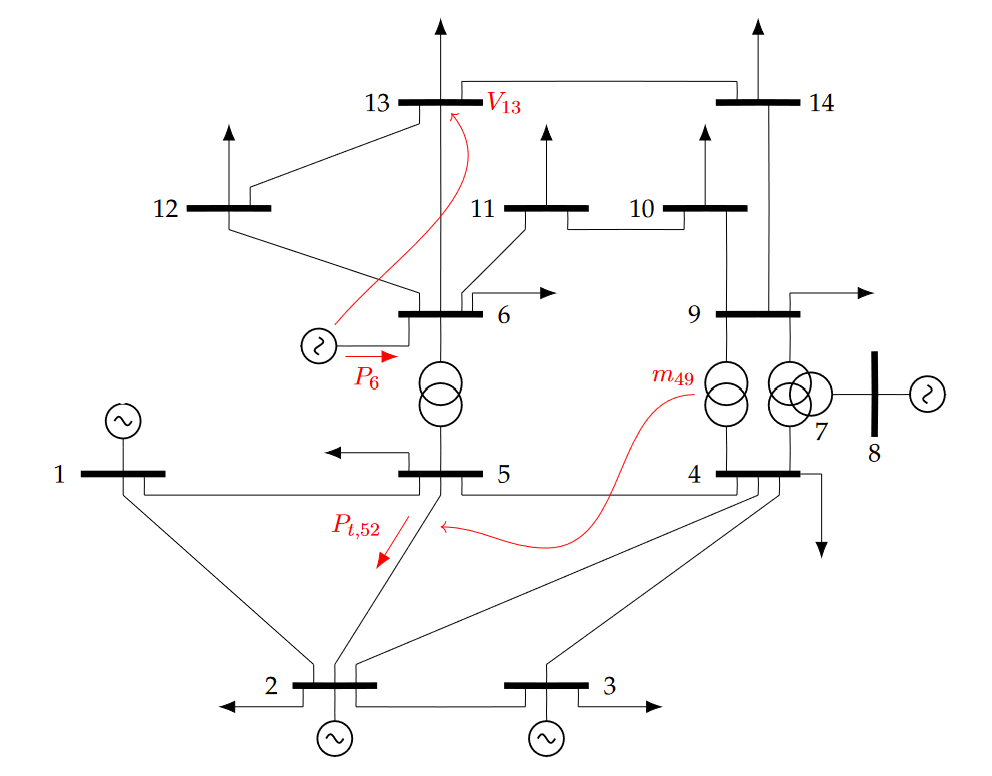
\includegraphics[width=0.9\textwidth]{chapter5pics/remote.png}
                \caption{Remote controls in IEEE 14-bus grid.}
                \label{fig:simple6bus}
            \end{figure}
        \end{column}
    \end{columns}
\end{frame}






% \begin{frame}{Sets for Known and Unknown Magnitudes}
%     \begin{table}[!htb]
%         \centering
%         \caption{Sets to identify known and unknown magnitudes.}
%         \begin{tabular}{cl}
%             \hline
%             \textbf{Set} & \textbf{Description} \\
%             \hline
%             $I_{\delta}$ & Known bus voltage phase \\
%             $I_{V}$ & Known bus voltage magnitudes \\
%             $I_{p}$ & Known bus ZIP active powers \\
%             $I_{q}$ & Known bus ZIP reactive powers \\
%             $K_{\tau}$ & Known branch tap phase shift angles \\
%             $K_{m}$ & Known branch tap ratios \\
%             $K_{p_{f}}$ & Known branch from active powers \\
%             $K_{p_{t}}$ & Known branch to active powers \\
%             $K_{q_{f}}$ & Known branch from reactive powers \\
%             $K_{q_{t}}$ & Known branch to reactive powers \\
%             $\overline{I}_{\delta}$ & Unknown bus voltage phase \\
%             $\overline{I}_{V}$ & Unknown bus voltage magnitudes \\
%             \hline
%         \end{tabular}
%         \label{tab:setsver2}
%     \end{table}
% \end{frame}
% \begin{frame}{Buses and Lines}
%     The sets $\mathcal{AC}$ and $\mathcal{DC}$ represent the bus indices for AC and DC buses, respectively. 
%     At first, all bus voltage magnitudes and phase angles are unknown, while ZIP powers are known.
    
%     \begin{align*}
%         \overline{I}_{V} &= \{\forall i \in \mathcal{AC} \cup \mathcal{DC} \}  \\
%         \overline{I}_\delta &= \{\forall i \in \mathcal{AC} \} \\
%         I_{\text{p}} &= \{\forall i \in \mathcal{AC} \cup \mathcal{DC} \}  \\
%         I_{\text{q}} &= \{\forall i \in \mathcal{AC} \} \\
%     \end{align*}
% \end{frame}
% \begin{frame}{ZIP Elements}
%     For buses with controllable ZIP elements (generators, SVCs, STATCOMs, etc.), their indices are moved from the known to the unknown sets.

%     \begin{align*}
%         GEN &= \{ \forall i \mid \text{bus i has a generator}\} \\
%         GEN_{AC} &= \{ i \in GEN \mid i \text{is an AC bus} \} \\
%         I_p &= I_p \setminus GEN \\
%         I_q &= I_q \setminus GEN_{AC} \\
%         \overline{I}_p &= \overline{I}_p \cup GEN \\
%         \overline{I}_q &= \overline{I}_q \cup GEN_{AC} \\
%     \end{align*}
% \end{frame}
% \begin{frame}{AC/DC Link - VSCs}
%     The set $ACDC$ contains branches representing AC/DC converters. We update the indices to include unknown active and reactive powers:

%     \begin{align*}
%         \overline{K}_{pf} &= \overline{K}_{pf} \cup \left\{ k \,\middle|\, k \in ACDC \right\} \\
%         \overline{K}_{pt} &= \overline{K}_{pt} \cup \left\{ k \,\middle|\, k \in ACDC \right\} \\
%         \overline{K}_{qt} &= \overline{K}_{qt} \cup \left\{ k \,\middle|\, k \in ACDC \right\} \\
%     \end{align*}
% \end{frame}
% \begin{frame}{Controllable Transformers}
%     The set $TR$ contains controllable transformers. Unknowns include powers, tap ratio, and phase shift.

%     \begin{align*}
%         \overline{K}_{pf} &= \overline{K}_{pf} \cup \left\{ k \,\middle|\, k \in TR \right\} \\
%         \overline{K}_{qf} &= \overline{K}_{qf} \cup \left\{ k \,\middle|\, k \in TR \right\} \\
%         \overline{K}_{pt} &= \overline{K}_{pt} \cup \left\{ k \,\middle|\, k \in TR \right\} \\
%         \overline{K}_{qt} &= \overline{K}_{qt} \cup \left\{ k \,\middle|\, k \in TR \right\} \\
%         \overline{K}_{\tau} &= \overline{K}_{\tau} \cup \left\{ k \,\middle|\, k \in TR \right\} \\
%         \overline{K}_{m} &= \overline{K}_{m} \cup \left\{ k \,\middle|\, k \in TR \right\} \\
%     \end{align*}
% \end{frame}
% \begin{frame}{Bus and Branch Setpoints}
%     Active elements asserting nodal or branch values move their indices from the unknown sets to the known sets:

%     \begin{align*}
%         I_{V} &= I_{V} \cup \{i\}, & \overline{I}_{V} &= \overline{I}_{V} \setminus \{i\} \\
%         I_{\delta} &= I_{\delta} \cup \{i\}, & \overline{I}_{\delta} &= \overline{I}_{\delta} \setminus \{i\} \\
%         K_{\tau} &= K_{\tau} \cup \{k\}, & \overline{K}_{\tau} &= \overline{K}_{\tau} \setminus \{k\} \\
%         K_{m} &= K_{m} \cup \{k\}, & \overline{K}_{m} &= \overline{K}_{m} \setminus \{k\} \\
%     \end{align*}
% \end{frame}
% \begin{frame}{Reference Node Identification}
%     Each connected system needs reference nodes:
%     \begin{itemize}
%         \item AC subsystems: At least one known phase angle and one known voltage magnitude.
%         \item DC subsystems: At least one known voltage magnitude.
%     \end{itemize}
%     These reference nodes are identified during the Depth-First Search (DFS) traversal.
% \end{frame}
% \begin{frame}{Identifying Connected Components (DFS)}
%     To identify subsystems, DFS is used to traverse the graph and find connected nodes. During traversal:
%     \begin{itemize}
%         \item Update connected nodes in set $B_j$.
%         \item Check if each node has known voltage/angle and update the reference sets $R_{\delta j}$, $R_{V j}$, and $R_{DC j}$.
%     \end{itemize}
% \end{frame}
% \begin{frame}{Cardinality of Unknown Sets}
%     Ensure the number of unknowns equals the number of equations. For example:
%     \begin{itemize}
%         \item Generators: 2 unknowns, 2 assertions, no new equations.
%         \item Controllable Transformers: 6 unknowns, 2 assertions, 4 new equations.
%         \item AC/DC Link: 3 unknowns, 2 assertions, 1 new equation.
%     \end{itemize}
% \end{frame}








% \subsection{Optimization theory}

% \begin{frame}{Non-linear optimization problem}
    
%     The general form of a non-linear optimization problem is given by:

%     \begin{equation}
%         \begin{split}
%             \text{min} \quad & f(\bm{x}) \\
%             \text{s.t.} \quad & \bm{G}(\bm{x}) = \bm{0} \\
%             & \bm{H}(\bm{x}) \leq \bm{0}
%         \end{split}
%     \end{equation}
%     \begin{itemize}
%         \item $\bm{x} \in \mathbb{R}^n$: Decision variables 
%         \item $f(x)$: Objective function 
%         \item $\bm{G}(\bm{x})$: Set of $n_e$ equality constraints
%         \item $\bm{H}(\bm{x})$: Set of $n_i$ inequalities. It is transformed into an equality using slack variables $Z_i \in \mathbb{R}^{+}$, such that $\bm{H}(\bm{x}) + \bm{Z} = \bm{0}$.
%     \end{itemize}
%     The associated Lagrangian function is given by:
%     \begin{equation}
%         \mathcal{L}(\bm{x}, \bm{Z}, \bm{\lambda}, \bm{\mu}) = f(\bm{x}) + \bm{\lambda}^\top \bm{G}(\bm{x}) + \bm{\mu}^\top (\bm{H}(\bm{x})+\bm{Z}) - \gamma \sum_{i=1}^{n_i} \log(z_i) 
%     \end{equation}

% \end{frame}


% \begin{frame}{KKT conditions}
%     The Karush-Kuhn-Tucker (KKT) conditions are necessary conditions for a solution to be optimal. They are given by:
%     \begin{equation}
%         \begin{split}            
%         \nabla_{x, Z, \lambda, \mu} \mathcal{L}(\bm{x}, \bm{Z}, \bm{\lambda}, \bm{\mu}) &= \bm{0} \\
%         \bm{\mathcal{L}}_x (\bm{x}, \bm{Z}, \bm{\lambda}, \bm{\mu}) &= \bm{f}_x + \bm{\lambda}^\top G_x + \bm{\mu}^\top H_x = \bm{0} \\
%         \bm{\mathcal{L}}_Z(\bm{x}, \bm{Z}, \bm{\lambda}, \bm{\mu}) &= \bm{\mu}^\top - \gamma \bm{1}_{n_i}^\top[\bm{Z}]^{-1} = \bm{0} \\
%         \bm{\mathcal{L}}_{\lambda}(\bm{x}, \bm{Z}, \bm{\lambda}, \bm{\mu}) &= \bm{G}^\top(\bm{x}) = \bm{0} \\
%         \bm{\mathcal{L}}_{\mu}(\bm{x}, \bm{Z}, \bm{\lambda}, \bm{\mu}) &= \bm{H}^\top(\bm{x}) + \bm{Z}^\top = \bm{0}\\ 
%         Z_i, \mu_i \geq 0 \quad \forall i 
%         \end{split}
% %         \label{eq:block1}
%     \end{equation}
    
%     %where $\bm{J}_G(\bm{x})$ and $\bm{J}_H(\bm{x})$ are the Jacobian matrices of $\bm{G}(\bm{x})$ and $\bm{H}(\bm{x})$, respectively, and $\bm{\lambda}$ and $\bm{\mu}$ are the Lagrange multipliers associated with the equality and inequality constraints, respectively.

% \end{frame}

% \subsection{IPM solver}

% \newcommand{\ones}{\mathbf{1}}

% \begin{frame}{Newton-Raphson method (1)}
%     The solving algorithm is based on the Newton-Raphson method, as it scales well with the size of the problem. 
%     \begin{equation}
%         - \begin{bmatrix}
%         \bm{\mathcal{L}}_{xx} & \bm{0} & \bm{G}_x^\top(\bm{x}) & \bm{H}_x^\top(\bm{x}) \\ 
%         \bm{0} & [\bm{\mu}] & \bm{0} & [\bm{Z}] \\
%         \bm{G}_x(\bm{x}) & \bm{0} & \bm{0} & \bm{0} \\
%         \bm{H}_x(\bm{x}) & \bm{I} & \bm{0} & \bm{0}
%         \end{bmatrix}
%         \begin{bmatrix}
%         \bm{\Delta x} \\
%         \bm{\Delta Z} \\
%         \bm{\Delta \lambda} \\
%         \bm{\Delta \mu}
%         \end{bmatrix} = 
%         \begin{bmatrix}
%         \bm{\mathcal{L}}_x^\top \\
%         [\bm{\mu}] \bm{Z} - \gamma \bm{1}_{n_i} \\
%         \bm{G}(\bm{x}) \\
%         \bm{H}(\bm{x}) + \bm{Z}
%         \end{bmatrix}
%     \end{equation}

%     The system is reduced to the following system of equations:

%     \begin{equation}
%         \begin{bmatrix}
%             \bm{M} & \bm{G}_{x}^\top \\
%             \bm{G}_{x} & \bm{0}
%         \end{bmatrix}
%         \begin{bmatrix}
%             \Delta \bm{x} \\
%             \Delta \bm{\lambda}
%         \end{bmatrix}
%         =
%         \begin{bmatrix}
%             -\bm{N} \\
%             -\bm{G}(\bm{x})
%         \end{bmatrix}
%         \label{eq:red5} 
%         \end{equation}
  
%         and after solving its displacements, the rest are calculated as:

%         \begin{equation}
%             \begin{split}
%                 \Delta \bm{\mu} &= -\bm{\mu} + \left[ \bm{Z} \right]^{-1} (\gamma \ones_{n_i}  - \left[ \bm{\mu} \right] \Delta \bm{Z})\\
%                 \Delta \bm{Z} &= -\bm{H}(\bm{X}) - \bm{Z} - \bm{H}_x \Delta \bm{X}
%             \end{split}
%             \label{eq:red6}
%         \end{equation}

% \end{frame}

% \begin{frame}{Newton-Raphson method (2)}
%     The updating process is performed using the following sequence of equations:
%     \begin{equation}
%         \begin{split}
%             \alpha_p &= \min \left( \tau \cdot \min \left(- \frac{\bm{Z}}{\Delta\bm{Z}}\right), 1 \right) \\
%             \alpha_d &= \min \left( \tau \cdot \min \left(- \frac{\bm{\mu}}{\Delta\bm{\mu}}\right), 1 \right)
%         \end{split}
%         \label{eq:step_length}
%     \end{equation}

%     \begin{equation}
%         \begin{split}
%             \bm{x} &\leftarrow \bm{x} + \alpha\alpha_p \Delta \bm{x} \\
%             \bm{Z} &\leftarrow \bm{Z} + \alpha\alpha_p \Delta \bm{Z} \\
%             \bm{\lambda} &\leftarrow \bm{\lambda} + \alpha\alpha_d \Delta \bm{\lambda} \\
%             \bm{\mu} &\leftarrow \bm{\mu} + \alpha\alpha_d \Delta \bm{\mu}
%         \end{split}
%         \label{eq:update}
%     \end{equation}
%     \begin{equation}
%         \gamma \leftarrow \sigma\frac{\bm{Z}^\top \bm{\mu}}{n_i}
%         \label{gamma_update}
%     \end{equation}

% \end{frame}
    
% \subsection{AC-OPF formulation}

% \begin{frame}{AC-OPF formulation - Variables and Objective Function}
%     The state vector of the problem has size $NV = 2n + 2n_g + 2m + 2n_{pq} + n_{m_p} + n_{\tau} + n_{DC}$ and is given by:
%     \begin{equation}
%         \bm{x} = [\textcolor{green}{\bm{\theta}^\top}, \textcolor{green}{\bm{\mathcal{V}}^\top}, \textcolor{green}{\bm{P}_g^\top}, \textcolor{green}{\bm{Q}_g^\top}, \bm{sl}_{sf}^\top, \bm{sl}_{st}^\top, \bm{sl}_{vmax}^\top, \bm{sl}_{vmin}^\top, \bm{m}_p^\top, \bm{\tau}^\top, \bm{P}_{DC}^\top]^\top
%     \end{equation}

%     where the green colored variables are the traditional AC-OPF variables. 

%     \begin{itemize}
%         \item $n$: Number of buses
%         \item $n_g$: Number of generators
%         \item $m$: Number of monitored branches
%         \item $n_{pq}$: Number of PQ buses
%         \item $n_{m_p}$: Number of module controlled transformers
%         \item $n_{\tau}$: Number of phase controlled transformers
%         \item $n_{DC}$: Number of DC lines
%     \end{itemize}
% \vspace{0.5cm}

%     The objective function of the problem is a quadratic cost function:
%     \begin{equation}
%         %\begin{split}
%             f(\bm{x}) = \sum_{i \in \text{ig}} c_{i_0} + c_{i_1}P_{g_i} + c_{i_2}P_{g_i}^{2} + \sum_{k \in \text{M}} c_{s_k} (sl_{sf_k} + sl_{st_k}) + \sum_{i \in \text{pq}} c_{{sl_v}_i} (sl_{vmax_i} + sl_{vmin_i})
%         %\end{split}
%     \end{equation}
% \vspace{1.5cm}
% \end{frame}
   
% \begin{frame}{AC-OPF formulation - Constraints}
%     The equality constraints contain the physical laws of the system as well as some of the fixed setpoints of the system
%     \begin{equation}
%     \begin{split}
%         \bm{G}(\bm{x}) = \begin{bmatrix}
%             \bm{G}^{S}_{P},&
%             \bm{G}^{S}_{Q},&
%             \bm{G}^{Th}_{slack},&
%             \bm{G}^{V}_{pv}
%             \end{bmatrix}
%     \end{split}
% \end{equation}

% with $\bm{G}^{S}_{P}$ and $\bm{G}^{S}_{Q}$ the active and reactive part of the power balance equations, $\bm{G}^{S}_{bus} = \bm{S}_{bus} - \bm{S}_{bus}^{g} + \bm{S}_{bus}^{d}  = \bm{0}$, $\bm{G}^{Th}_{slack}$ the slack bus angle, and $\bm{G}^{V}_{pv}$ the voltage constraints of the PV buses.
% \vspace{0.5cm}

% The inequality constraints are those which take into account the operational limits of the grid, as well as the auxiliary slack variables limitations:
% \begin{equation}
%     \begin{split}
%         \bm{H}(\bm{x}) = \left[ \right.& \bm{H}^{S_f}, \bm{H}^{S_t}, \bm{H}^{V_u}, \bm{H}^{P_u}, \bm{H}^{Q_u}, \bm{H}^{V_l}, \bm{H}^{P_l}, \bm{H}^{Q_l}, \bm{H}^{sl} \\
%         &\left.  \bm{H}^{m_{p_u}}, \bm{H}^{m_{p_l}}, \bm{H}^{\tau_u}, \bm{H}^{\tau_l}, \bm{H}^{Q_{max}}, \bm{H}^{P_{DC_u}}, \bm{H}^{P_{DC_l}} \right]
%     \end{split}
% \end{equation}

% All the first and second derivatives for the constraints necessary for the jacobian matrix of the Newton-Raphson are described in the thesis.

% \end{frame}
